\documentclass{article}
\usepackage{amsmath}
\usepackage{amssymb}
\usepackage{tikz}
\usepackage{xspace}
\usepackage{float}
\usepackage{circuitikz}
\usepackage{physics}
\usepackage{tikz}
\newcommand*\circled[1]{\tikz[baseline=(char.base)]{
   \node[shape=circle,draw,inner sep=1pt] (char) {#1};}}
\newcommand*\electron{\mathrm{e}^-}
\usepackage{paracol}

\title{AP Physics C: Chapter 24}
\author{Zach Baylin}

\begin{document}
  \maketitle
  \section{Gauss' Law}
    \begin{itemize}
      \item Symmetry remains important
      \item Symmetry of $E_1$ \textit{must} be similar symmetry of charge distribution
        \begin{itemize}
          \item cylindrical - infinitely long
          \item planar - infinitely wide
          \item spherical
        \end{itemize}
      \item \underline{Flux $(\Phi_E)$}: amount of electric field lines that pass through a surface\\
        \begin{center}
          
\begin{tikzpicture}
            \draw[->] (0,0) -- (2,0);
            \draw[->] (0,.25) -- (2,.25);
            \draw[->] (0,.5) -- (2,.5);
            \node at (4,.25) {implies charge};
            \node at (2.5,.25) {$E$};
          \end{tikzpicture}
        \end{center}
      \item if $\Phi_{E}$ is only in, $q_{\text{net}}=(-)$
      \item if $\Phi_{E}$ is only out, $q_{\text{net}}=(+)$
      \item if in matches out $q_{\text{net}}=\phi$
      \item imaginary surface = Gaussian surface encloses a region of space around a charge\\
        \begin{paracol}{3}
          \begin{center}
            Net $q-$\\~\\
            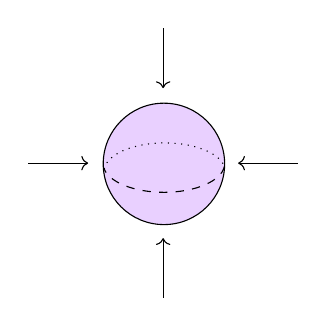
\begin{tikzpicture}[x=0.75pt,y=0.75pt,yscale=-1,xscale=1]
              \draw  [fill={rgb, 255:red, 144; green, 19; blue, 254 }  ,fill opacity=0.2 ] (36.13,65.36) .. controls (36.13,49.21) and (49.23,36.11) .. (65.38,36.11) .. controls (81.54,36.11) and (94.63,49.21) .. (94.63,65.36) .. controls (94.63,81.52) and (81.54,94.61) .. (65.38,94.61) .. controls (49.23,94.61) and (36.13,81.52) .. (36.13,65.36) -- cycle ;
              \draw  [draw opacity=0][dashed] (94.52,66.51) .. controls (93.19,73.54) and (80.65,79.06) .. (65.37,79.06) .. controls (51.05,79.06) and (39.13,74.21) .. (36.6,67.8) -- (65.37,65.27) -- cycle ; \draw  [dashed] (94.52,66.51) .. controls (93.19,73.54) and (80.65,79.06) .. (65.37,79.06) .. controls (51.05,79.06) and (39.13,74.21) .. (36.6,67.8) ;
              \draw  [draw opacity=0][dotted] (36.6,67.8) .. controls (37.93,60.77) and (50.47,55.25) .. (65.75,55.25) .. controls (80.07,55.25) and (92,60.1) .. (94.52,66.51) -- (65.75,69.04) -- cycle ; \draw  [dotted] (36.6,67.8) .. controls (37.93,60.77) and (50.47,55.25) .. (65.75,55.25) .. controls (80.07,55.25) and (92,60.1) .. (94.52,66.51) ;
              \draw[<-]    (101.11,65) -- (130,65) ;
              \draw[<-]    (65,101.11) -- (65,130) ;
              \draw[->]    (0,65) -- (28.89,65) ;
              \draw[<-]    (65,28.89) -- (65,0) ;
            \end{tikzpicture}
          \end{center}
          \switchcolumn
          \begin{center}
            Net $q=0$\\~\\
            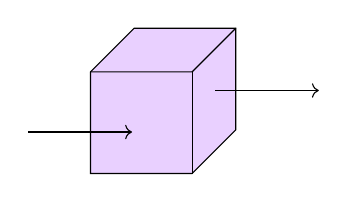
\begin{tikzpicture}[x=0.75pt,y=0.75pt,yscale=-1,xscale=1]
              \draw  [fill={rgb, 255:red, 144; green, 19; blue, 254 },fill opacity=0.2 ] (30,41) -- (51,20) -- (100,20) -- (100,69) -- (79,90) -- (30,90) -- cycle ; \draw   (100,20) -- (79,41) -- (30,41) ; \draw   (79,41) -- (79,90) ;
              %Straight Lines [id:da004591705395383228] 
              \draw[<-]    (50,70) -- (0,70) ;
              %Straight Lines [id:da18489965033627564] 
              \draw[->]    (90,50) -- (140,50) ;
            \end{tikzpicture}
          \end{center}
          \switchcolumn
          \begin{center}
            Net $q+$\\~\\
            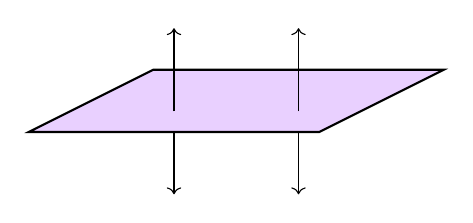
\begin{tikzpicture}[x=0.75pt,y=0.75pt,yscale=-1,xscale=1]
              \draw  [color={rgb, 255:red, 0; green, 0; blue, 0 }  ,draw opacity=1 ][fill={rgb, 255:red, 144; green, 19; blue, 254 }  ,fill opacity=0.2 ][line width=0.75]  (70,30) -- (210,30) -- (150,60) -- (10,60) -- cycle ;
              \draw[->]    (140,50) -- (140,10) ;
              \draw[->]    (80,50) -- (80,10) ;
              \draw[<-]    (80,90) -- (80,60) ;
              \draw[<-]    (140,90) -- (140,60) ;
            \end{tikzpicture}

          \end{center}
        \end{paracol}
      \item choose the Gaussian surface closest to the symmetry of the distribution
        \begin{itemize}
          \item point charge \rightarrow\xspace sphere
          \item cylinder \rightarrow\xspace cylinder
          \item cylinder \rightarrow\xspace plane
        \end{itemize}
      \item ex.
        \begin{center}
          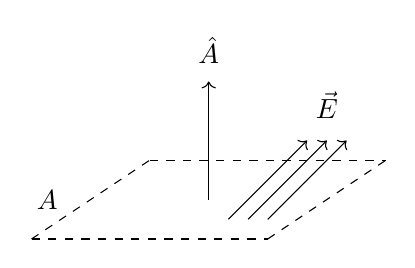
\begin{tikzpicture}
            \draw[dashed] (0,0) -- (3,0);
            \draw[dashed] (1.5,1) -- (4.5,1);
            \draw[dashed] (0,0) -- (1.5,1);
            \draw[dashed] (3,0) -- (4.5,1);
            \draw[->] (2.25, .5) -- (2.25, 2);
            \draw[->] (2.5, .25) -- (3.5, 1.25);
            \draw[->] (2.75, .25) -- (3.75, 1.25);
            \draw[->] (3, .25) -- (4, 1.25);
            \node at (2.25, 2.4) {$\hat{A}$};
            \node at (3.75, 1.7) {$\vec{E}$};
            \node at (.2, .5) {$A$};
          \end{tikzpicture}
        \end{center}
      \item $\phi_{E}=\vec{E}\cdot\vec{A}=|E||A|\cos(\theta)$
      \item $\phi_{E}=\int_{\text{Surface}}\vec{E}\cdot \dd{A}=\int|E|\cos\theta \dd{A}=EA\cos\theta$
      \item \underline{Closed Surface}: a surface that is contained
      \begin{itemize}
        \item $\Phi_E = \oint\vec{E}\cdot \dd{\vec{A}}$
        \item ex.
          \begin{center}
            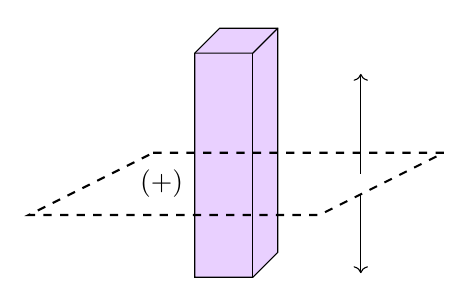
\begin{tikzpicture}[x=0.75pt,y=0.75pt,yscale=-1,xscale=1]
              \draw  [fill={rgb, 255:red, 144; green, 19; blue, 254 }  ,fill opacity=0.2] (80,12) -- (92,0) -- (120,0) -- (120,108) -- (108,120) -- (80,120) -- cycle ; \draw   (120,0) -- (108,12) -- (80,12) ; \draw   (108,12) -- (108,120) ;
              \draw  [color={rgb, 255:red, 0; green, 0; blue, 0 }  ,draw opacity=1 ][dashed][line width=0.75]  (60,60) -- (200,60) -- (140,90) -- (0,90) -- cycle ;
              \draw[->]    (160,70) -- (160,22) ;
              \draw[->]    (160,80) -- (160,118);
              \draw (64,75) node  [align=left] {(+)};
              \end{tikzpicture}
          \end{center}
      \end{itemize}
      \item \textbf{Summary}:
        \begin{itemize}
          \item $\hat{A}=$ normal to the surface of area $A$
          \item $E_\perp$ to the surface and has the same magnitude, then $\vec{E}\cdot \dd{\vec{A}=EA}$
          \item $\Phi_E$ is \textsc{max} when $\theta=0$ when $E_\perp$ to the surface
          \item $\Phi_E=0$ when $\theta=90^\circ=\dfrac{\pi}{4}$
        \end{itemize}
      \item ex. for two point charges:
      \begin{center}
        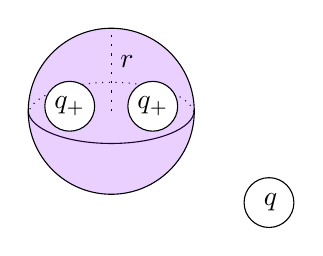
\begin{tikzpicture}[x=0.75pt,y=0.75pt,yscale=-.8,xscale=.8]
          %uncomment if require: \path (0,135); %set diagram left start at 0, and has height of 135
          
          %Shape: Arc [id:dp7179008660290112] 
          \draw  [draw opacity=0][dotted] (0.02,52.59) .. controls (0.02,41.55) and (22.41,32.59) .. (50.02,32.59) .. controls (77.14,32.59) and (99.22,41.23) .. (100,52) -- (50.02,52.59) -- cycle ; \draw  [dotted] (0.02,52.59) .. controls (0.02,41.55) and (22.41,32.59) .. (50.02,32.59) .. controls (77.14,32.59) and (99.22,41.23) .. (100,52) ;
          %Shape: Arc [id:dp34328570930088564] 
          \draw  [draw opacity=0] (99.98,49.41) .. controls (99.98,60.45) and (77.59,69.41) .. (49.98,69.41) .. controls (22.86,69.41) and (0.78,60.77) .. (0,50) -- (49.98,49.41) -- cycle ; \draw   (99.98,49.41) .. controls (99.98,60.45) and (77.59,69.41) .. (49.98,69.41) .. controls (22.86,69.41) and (0.78,60.77) .. (0,50) ;
          %Shape: Circle [id:dp46577421003546005] 
          \draw  [fill={rgb, 255:red, 144; green, 19; blue, 254 }  ,fill opacity=0.2 ] (0,50) .. controls (0,22.39) and (22.39,0) .. (50,0) .. controls (77.61,0) and (100,22.39) .. (100,50) .. controls (100,77.61) and (77.61,100) .. (50,100) .. controls (22.39,100) and (0,77.61) .. (0,50) -- cycle ;
          %Shape: Circle [id:dp6064672046482136] 
          \draw  [fill={rgb, 255:red, 255; green, 255; blue, 255 }  ,fill opacity=1 ] (60,47) .. controls (60,38.72) and (66.72,32) .. (75,32) .. controls (83.28,32) and (90,38.72) .. (90,47) .. controls (90,55.28) and (83.28,62) .. (75,62) .. controls (66.72,62) and (60,55.28) .. (60,47) -- cycle ;
          %Shape: Circle [id:dp36253140102891757] 
          \draw  [fill={rgb, 255:red, 255; green, 255; blue, 255 }  ,fill opacity=1 ] (10,47) .. controls (10,38.72) and (16.72,32) .. (25,32) .. controls (33.28,32) and (40,38.72) .. (40,47) .. controls (40,55.28) and (33.28,62) .. (25,62) .. controls (16.72,62) and (10,55.28) .. (10,47) -- cycle ;
          %Straight Lines [id:da8854125283346765] 
          \draw  [dash pattern={on 0.84pt off 2.51pt}]  (50,50) -- (50,0) ;
          
          
          %Shape: Circle [id:dp6135994022576992] 
          \draw   (130,105) .. controls (130,96.72) and (136.72,90) .. (145,90) .. controls (153.28,90) and (160,96.72) .. (160,105) .. controls (160,113.28) and (153.28,120) .. (145,120) .. controls (136.72,120) and (130,113.28) .. (130,105) -- cycle ;
          
          % Text Node
          \draw (75,47) node  [align=left] {$\displaystyle q_{+}$};
          % Text Node
          \draw (25,47) node  [align=left] {$\displaystyle q_{+}$};
          % Text Node
          \draw (59.5,20) node  [align=left] {$\displaystyle r$};
          % Text Node
          \draw (146,105) node  [align=left] {$\displaystyle q$};
        \end{tikzpicture}\\          
        surround both in a single sphere
      \end{center}
      \item Charge densities:
        \begin{itemize}
          \item \textbf{Linear Charge Density ($\lambda$)}: $\dfrac{Q}{L}$
          \item \textbf{Area Charge Density ($\sigma$)}: $\dfrac{Q}{A}$
          \item \textbf{Volume Charge Density ($\rho$)}: $\dfrac{V}{A}$
        \end{itemize}
      \item Electric field as distance increases:
        \begin{center}
          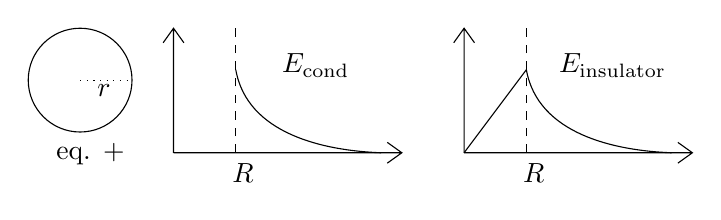
\begin{tikzpicture}[x=0.75pt,y=0.75pt,yscale=-1,xscale=1]
            \draw   (0,25) .. controls (0,11.19) and (11.19,0) .. (25,0) .. controls (38.81,0) and (50,11.19) .. (50,25) .. controls (50,38.81) and (38.81,50) .. (25,50) .. controls (11.19,50) and (0,38.81) .. (0,25) -- cycle ;
            \draw  [dotted]  (25,25) -- (50,25) ;
            \draw  (70,60) -- (180,60)(70,0) -- (70,60) -- cycle (173,55) -- (180,60) -- (173,65) (65,7) -- (70,0) -- (75,7)  ;
            \draw    (100,20) .. controls (105.5,51) and (142.5,59) .. (170,60) ;
            \draw  (210,60) -- (320,60)(210,0) -- (210,60) -- cycle (313,55) -- (320,60) -- (313,65) (205,7) -- (210,0) -- (215,7)  ;
            \draw    (240,20) .. controls (245.5,51) and (282.5,59) .. (310,60) ;
            \draw    (210,60) -- (240,20) ;
            \draw  [dashed]  (100,60) -- (100,0) ;
            \draw  [dashed]  (240,60) -- (240,0) ;
            \draw (36.5,30) node  [align=left] {$\displaystyle r$};
            \draw (103.5,70) node  [align=left] {$\displaystyle R$};
            \draw (243.5,70) node  [align=left] {$\displaystyle R$};
            \draw (30,60.5) node  [align=left] {eq. $\displaystyle +$};
            \draw (138.5,18) node  [align=left] {$\displaystyle E_{\text{cond}}$};
            \draw (281.5,18) node  [align=left] {$\displaystyle E_{\text{insulator}}$};
          \end{tikzpicture}
        \end{center}
    \end{itemize}
  \section{Capacitors}
    \begin{center}
      \includegraphics{figures/capacitor.pdf}
    \end{center}
    \begin{itemize}
      \item Work done on a charge $q$ in a constant electric field $E$
        \begin{align*}
          F_E&=qE\\
           &=q\dfrac{V}{d}\\
          W_\text{done}=F_E\cdot d& =q\Delta V = \Delta k\\~\\
          W&=\Delta k\\
          W_\text{done by external force}&=\Delta U_E\\
          W_\text{done by field}&=-\Delta U_E
        \end{align*}
      \item Objects with non-constant $E$
        \begin{itemize}
          \item point charge
          \item sphere
          \item rod
        \end{itemize}
      \item To solve with non-constant $E$
        \begin{itemize}
          \item Find $E$, either using superposition or Gauss' law
          \item Find $\Delta V=\oint E\cdot \dd r$
        \end{itemize}
      \item Electic field is the negative slope of potential: $E=\dfrac{- \dd v}{\dd r}$
      \item Calculating $U_E$
        \begin{figure}[H]
          \centering
          \includegraphics{figures/calculating-ue.pdf}
          \caption{A diagram of $U_e$}
        \end{figure}
    \end{itemize}
  \section{Capacitors}
    \begin{figure}[H]
      \centering
      \includegraphics{figures/metal-plates.pdf}
      \caption{A diagram of metal plates}
    \end{figure}
    \begin{itemize}
      \item \textbf{Capacitor} - stores charge/electric energy
      \item \textbf{Parallel plates}
        \begin{figure}[H]
          \centering
          \includegraphics{figures/parallel-plates.pdf}
          \caption{A diagram of parallel plates}
        \end{figure}
      \item To find the electric potential between the plates:
        \begin{align*}
          \Delta V= V_\mathrm{f}-V_\mathrm{i}=&-\int_0^x E\cdot\dd s\\
           &=-\int_0^x \dfrac{-Q}{\varepsilon_0 A}\cdot x\\
           &=\dfrac{Q}{\varepsilon_0 A}\cdot x\\
           &=\dfrac{Q}{\varepsilon_0 A}\cdot d\\
        \end{align*} 
      \item \textbf{Capacitance}: ratio of charge to change in electric potential
        \begin{figure}[H]
          \centering
          \includegraphics{figures/capacitance-graph.pdf}
          \caption{A plot demonstrating capacitance}
        \end{figure}
      \item \textbf{Dialectric}: insulator between plates polarizes to create an $\vec{E}$ opposite $E_C$
      \item \textbf{Dialectric constant}: $K=\dfrac{E_0}{E}$
        \begin{itemize}
          \item air: $\approx1$
          \item water: $\approx80$
        \end{itemize}
      \item Amt. of charge is a function of the capacitance and the battery: $Q=C\Delta V$
      \item 
    \end{itemize}
\end{document}
